\documentclass{article}
\usepackage{amsmath}
\usepackage{amssymb}
\usepackage{listings}
\usepackage{graphicx}
\begin{document}
\noindent Let $ (R_1,R_2) \in \mathbb{R^2} $ two resistance values of two resistor $r_1$ and $r_2$. Let $ (\epsilon_1,\epsilon2) \in \mathbb{R^2} $ their tolerance values.\\
If $r_1$ and $r_2$ are in parallel: \\
- The first algebraic relation is: $ R_{par} = \frac{R_1*R_2}{R_1 + R_2} $\\
$\implies \epsilon_{par} =  \frac{(R_1+\epsilon_1)(R_2+\epsilon_2)}{(R_1 + R_2) + (\epsilon_1 + \epsilon_2)} -  \frac{R_1*R_2}{R_1 + R_2} $\\
- The second algebraic relation is: $R_{par} = \frac{1}{\frac{1}{R_1} + \frac{1}{R_2}} $\\
$\implies \epsilon_{par} =  \frac{1}{\frac{1}{R_1+\epsilon_1} + \frac{1}{R_2+\epsilon_2}} - \frac{1}{\frac{1}{R_1} + \frac{1}{R_2}}$\\
Given the two scheme functions $par1$ and $par2$ :\\
\begin{lstlisting}
  (define (div-interval x y)
     (cond ((= (width y) 0)
             (error "can't divide by an interval of width 0")))
; the old  implementation inverts lower and upper bound
;          (mul-interval x
;	          (make-interval (/ 1.0 (upper-bound y))
;	           		 (/ 1.0 (lower-bound y)))))
      (make-interval (/ (lower-bound x) (lower-bound y))
                     (/ (upper-bound x) (upper-bound y))))
  
  (define (par1 r1 r2)
     (div-interval (mul-interval r1 r2)
                   (add-interval r1 r2)))

  (define (par2 r1 r2)
     (let ((unit (make-interval 1.0 1.0)))
        (div-interval unit
		      (add-interval (div-interval unit r1)
				    (div-interval unit r2)))))
\end{lstlisting}


\noindent The algebraic relations both give the same error. Our calculations in \texttt{par1} and \texttt{par2} break from the algebraic notions  of an interval as we will show.\\
Lets try to write the \texttt{lower-bound} and \texttt{upper-bound} in terms of the two forms of a parallel resistance (or how \texttt{par1} and \texttt{par2} calculate them).\\ \\
Let $u_{r} , l_{r}$ respectively be the upper and lower bounds of an interval $r$ and let $U_{r_1.r_2}$  be the upper bound for $R1.R2$ and let $L_{r_1.r_2}$ be the lower bound of $R1 . R2;$\\
\noindent$l_{par1} =  \frac{L_{r_1r_2}}{U_{r_1+ r_1}} < \frac{u_{r1}u_{r_2}}{U_{r_1+r_2}} $\\
\noindent$ l_{par2} = \frac{1}{\frac{1}{u_{r_1}} + \frac{1}{u_{r_2}}} > l_{par1} $\\
By symmetry of the proof, this can be also proven that $u_{par1} > u_{par2}$\\
$\implies \forall (r1,r2) \in \mathbb{N^2}, e_{par1} > e_{par_2} | e_{par1} = r1*r2 - l_{par1} = u_{par1} - r1*r2 $ AND $ e_{par2} = r1*r2 - l_{par2} = u_{par2} - r1*r2 $\\
\noindent The par2 procedure is more suitable for parallel resistances calculation because the division by the unit (1/r1 and 1/r2) doesn't create an expansion of the result unreasonably. While the multiplication of $R1*R2$ has that effect. In a sense par2 doesn't make the operation depend on an expansive multiplication of R1 and R2. It seems this is inherit to arithmetic operations over intervals, it is not trivial to define an exact arithmetic of intervals as it is dependent upon a function that might exhibit a minimum and a maximum not at the images of the extremeties of the intervals in question and not at extermeties that are written directly in function of the limits of the intervals in question.

\noindent In short the problem appears becase we assume that the minimum and the maximum of the algebraic equation will map directly to the minimum and maximum of the input intervals which is not necessarily the case. As algebraic equations can be thought of as functions who migh exhibit a maximum and a minimum way before the boundaries of an interval. The maximum and the minimum although might be related to the boundaries of the input intervals they might not relate to the partial composition of the total function from elementary arithmetic of the intervals. Addition, Substraction, multiplication and division of intervals when composed into larger functions will create other maximums and minimums than the ones treated in their elementary form. That is because functions follow an evolution different from the elementary operations that create them. Also functions might exhibit critical points away from the boundaries of the input intervals ..

\noindent We include a figure showing the divergeance between $par1$ and $par2$ .
\begin{figure}[htbp]
    \centering
    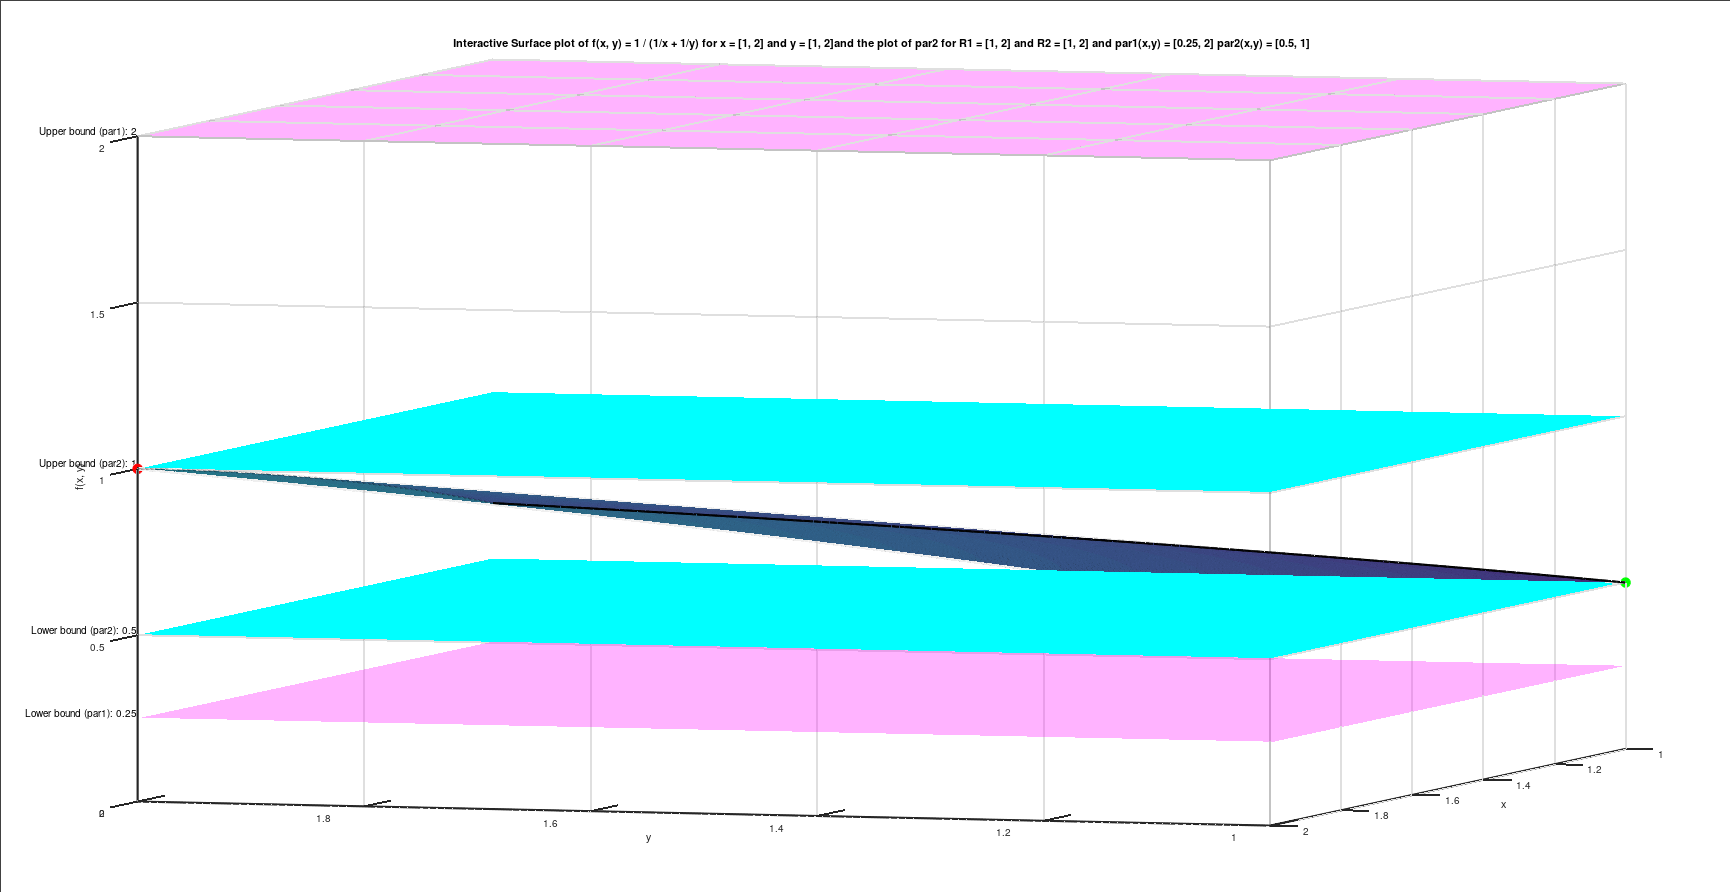
\includegraphics[width=\linewidth]{exe-2.15-diff-par1-par2.png}
    \caption{par1 vs par2 vs the two variables function 1/(1/x + 1/y).}
    \label{fig:yourlabel}
\end{figure}

\end{document} 
